%%++++++++++++++++++++++++++++++++++++++++++++++++++++++++++++++++++++++++++++
%%            INFORMATION
%%============================================================================
%%            Release
%%----------------------------------------------------------------------------
\def\CurrentVersionMain{\textit{V2.0}}
%%============================================================================
%%            Category of the document and praembel
%%----------------------------------------------------------------------------
\documentclass[12pt,a4paper,oneside,bibliography=totocnumbered,toc=listofnumbered]{scrbook}
\usepackage[ngerman,naustrian,english]{babel}
\usepackage{./packages/WissensArbeitenFHWels}
\usepackage{./packages/WissensArbeitenFHWels-FrontseitenEN}     

%%++++++++++++++++++++++++++++++++++++++++++++++++++++++++++++++++++++++++++++
%%
%%++++++++++++++++++++++++++++++++++++++++++++++++++++++++++++++++++++++++++++
%%            Specifications and settings of the academic thesis
%%============================================================================
%%            Specifications
%%----------------------------------------------------------------------------
%% Title of your academic work:
\title{>>Software Development for Controlling Glare-Free Adaptive High Beam in Matrix LED Pixel Headlight<<}
%%
%% Author of the thesis:
\author{>>T. Cagil Oral<<}
%%
%% Degree programme:
\studiengang{>>Automotive Mechatronics and Management<<}
%%
%% Type of document:
\typDokument{>>Master Thesis<<}
% -) "Bachelor thesis"
% -) "Master thesis"
% -) "project report"
%%
%% Type of degree:
\artStudiengang{>>Master's degree programme<<}
% -) "Bachelor's degree programme"
% -) "Master's degree programme"
%%
%% Title upon graduation:
\akademGrad{>>Master of Science in Engineering (MSc)<<}
% -) "Bachelor of Science in Engineering (BSc)"
% -) "Master of Science in Engineering (MSc)"
% -) "Diplom-Ingenieurin für technisch-wissenschaftliche Berufe (Dipl.-Ing.)"
% -) "Diplom-Ingenieur für technisch-wissenschaftliche Berufe (Dipl.-Ing.)"
%%
%% City of residence:
\studienort{>>Wels<<}
%%
%% Month and year of release
\abgabemonat{>>September<<}
\abgabejahr{>>2024<<}
%%
%% Supervisior:
\betreuer{>>Prof. Gerald Steinmaurer \\ Dr.Harald Kirchsteiger<<}
%%
%% Keywords for the thesis:
%% (for the metadatas of the PDF)
\stichwoerter{A, Stichwort 2 Stichwort 3...}
%%
%% Show signature: (ATTENTION: The syntax is important!!!)
\ShowSignature{0mm}{22mm}{0.5}{No}		% Shows the signature at the sworn decleration
% Syntax: {x-Position}{y-Position}{Scale factor}{'Show:' Yes / No}
% Example: \ShowSignature{0mm}{22mm}{0.5}{Yes}
% A file with the name "Signature.png" must exist in the folder for the graphics
%%
%% Show colored links: (ATTENTION: The syntax is important!!!)
\ColoredLinks{No}		% Colored links for figures, URLs and literature
% Syntax: Yes / No
%%
%%============================================================================
%%            Settings
%%----------------------------------------------------------------------------
\Style{FHWels}				% Defines the basic style (only 'FHWels possible)
\BibStyle{FHWelsNumericBrackets}	% Citation style based on'BibLatex
% Syntax:	-) FHWelsNumericBrackets (e.g. [1])
%			-) FHWelsAlphabeticBrackets (e.g. [Meier, 2011])
\addbibresource{Bibliography.bib}	% Bibliography file(s)


\graphicspath{{./Grafik/}}	% Sets the folder for the graphics
\TabContent{1.4cm}			% Tab stop for the list of content
%%++++++++++++++++++++++++++++++++++++++++++++++++++++++++++++++++++++++++++++
%%
%%++++++++++++++++++++++++++++++++++++++++++++++++++++++++++++++++++++++++++++
%%            BEGINNING OF THE THESIS
%%============================================================================
\begin{document}
\selectlanguage{english}	% Sets the language	
%%============================================================================
%%            Frontpages & sworn decleration
%%----------------------------------------------------------------------------
%% Titelseite
	\frontmatter				% roman page numbers				
	\pagenumbering{Roman}		% capital roman numbers
	\titelseite
%%	
%%============================================================================
%%            Pre-chapters
%%----------------------------------------------------------------------------
%% Preface, Kurzfassung/Abstract, Contents
	\begingroup
		\pagestyle{plain}				%...no headline
		\renewcommand{\chapterpagestyle}{plain}
		\chapter{Preface/Acknowledgements}
The preface contains a short description of the topic; words of thanks to companies, mentors, supervisors, family members, etc., for their support are optional under consideration of relevant data protection terms.

\section{Using this template}
This document is a template and contains optional lists. Lists that are not required (list of abbreviations, glossary, list of figures, list of tables and list of equations) may be deleted after consultation with your supervisor. Please discuss with your supervisor in advance which format, reference style, structure of chapters, etc. is to be used. Course-specific regulations might be included in an additional document. Please contact your supervisor on this matter.
\vspace{6pt}\\
The examples provided in this template are for your information only. Replace them with your own text after reading them carefully. Delete unnecessary information. Please keep in mind that automatic numbering is shown correctly in the document as a whole only after you have deleted sub-chapters of the preface which explains the template.
\vspace{6pt}\\
For an updated table of contents, the document should always be compiled twice.
\vspace{6pt}\\
\textcolor{red}{\textbf{The present format template was prepared to the best of our knowledge and judgement. However, it is used at the users’ own risk with regard to the possible loss of data, computer problems or financial and material damage which may result from the use of this template. The authors of the present format template and the University of Applied Sciences Upper Austria do not accept any liability for the correct functionality of this template.}}



\newpage
\subsection{Experience with \LaTeX}
Some experience with the software package {\LaTeX} is necessary for using this template. The program \textbf{TeXstudio} (\url{www.texstudio.org}) and the windows distribution \textbf{MiKTEX} (\url{www.miktex.org}) were used to create this template. Problems may arise when using other software. This template is not compatible with Apple operating systems.\\
The style packages used and the commands needed are not explained in this template. Detailed help for the commands is offered at the internet in many forums and websites.

\section{Headings}
With respect to headings, consider the following points for the formulation of a table of contents:
\begin{itemize}
	\item Do not use unknown abbreviations in headings
	\item No full stop at the end of headings
	\item Make sure that a heading – without associated text – is not situated on the last line of a page; a page should also not start with a single line which belongs to the paragraph on the previous page.
	\item The degree of detail corresponds to the focus and emphasis of the thesis
	\item Always use at least two sub-chapters in one chapter; otherwise do not use sub-chapters
	\item Use a maximum of 5 levels of sub-chapters
\end{itemize}
Due to the automatic structuring done by {\LaTeX} the headings can not be illustrated here, but the commands can be explained:
\begin{itemize}
	\item level of heading 1: \verb|\chapter{...}| command
	\item level of heading 2: \verb|\section{...}| command
	\item level of heading 3: \verb|\subsection{...}| command
	\item level of heading 4: \verb|\subsubsectin{...}| command
	\item level of heading 5: \verb|\paragraph{...}| command
\end{itemize}

\newpage
\section{Abbreviations}
{\LaTeX} automatically creates spaces between characters in some cases. For common abbreviations to be depicted in the right way, commands are defined.

\begin{multicols}{2}	
	\begin{itemize}
		\item Command: \verb|\mn|\dotfill\mn
		\item Command: \verb|\mx|\dotfill\mx
		\item Command: \verb|\etc|\dotfill\etc
		\item Command: \verb|\ie|\dotfill\ie
		\item Command: \verb|\eg|\dotfill\eg
		\item Command: \verb|\cf|\dotfill\cf
	\end{itemize}
\end{multicols}

\newpage
\section{Figures}
\label{sec: Figures}
The figure environment has to be used for inserting and referencing figures.\\
A figure can be inserted with the following lines of code:
\begin{figure}[h]
	\centering
	
\includegraphics[width=0.50\textwidth]{FH.png}
	\caption{Example of inserting a figure}
	\label{fig: ExampleFigure-1}
\end{figure}\\
Two figures next to each other with one caption can be inserted with the following commands:
\begin{figure}[htp!]
	\begin{minipage}[t]{0.49\textwidth}
		\centering
		
\includegraphics[width=0.49\textwidth]{FH.png}
	\end{minipage}
	\hfill
	\begin{minipage}[t]{0.49\textwidth}
		\centering
		
\includegraphics[width=0.49\textwidth]{FH.png}
	\end{minipage}
	\caption{Example of two figures with one caption}
	\label{fig: ExampleFigure-2}
\end{figure}\\
Two figures next to each other with separate captions can be inserted with the commands below:
\begin{figure}[htp!]
	\begin{minipage}[t]{0.49\textwidth}
		\centering
		
\includegraphics[width=0.49\textwidth]{FH.png}
		\caption{Examples of two figures with separate captions}
		\label{fig: ExampleFigure-3}
	\end{minipage}
	\hfill
	\begin{minipage}[t]{0.49\textwidth}
		\centering
		
\includegraphics[width=0.49\textwidth]{FH.png}
		\caption{Examples of two figures with separate captions}
		\label{fig: ExampleFigure-4}
	\end{minipage}
\end{figure}\\
Consider the following points when using figures:
\begin{itemize}
	\item Figures must be referenced within or linked to the text; otherwise they are superfluous. To do this, use the command \verb|\ref{}|
	[see Fig.~\ref{fig: ExampleFigure-1}]\\
	An additional page reference can be added with the command \verb|\pageref{}| \newline
	[see Fig.~\ref{fig: ExampleFigure-1} on page \pageref{fig: ExampleFigure-1}]
	\item Not every figure needs to be in the text. Analyses, tables, backup information, \etc can be collected in the appendix. However, the text should reference them.
	\item If necessary, add a legend in the figures and the necessary references.
\end{itemize}

\newpage
\section{Tables}
Tables must be referenced within or linked to the text [see Table \ref{tab: ExampleTable-1} on page~\pageref{tab: ExampleTable-1}].\\
Using the table environment, tables can be numbered and referenced correctly.\\
A table can be inserted in two different ways.
\subsection{Insert as a figure}
An image of a table can be inserted in the table environment.
\begin{table}[h]
	\centering
	\caption{Example of a table inserted as a figure}
	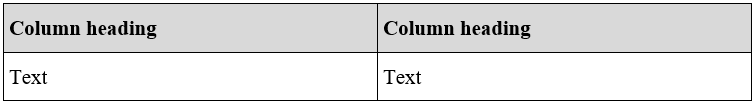
\includegraphics[scale=0.6]{0000_Testtabelle.png}
	\label{tab: ExampleTable-1} 
\end{table}
\subsection{Insert as a table}
It is possible to create tables with {\LaTeX} directly.
\begin{table}[h]
	\centering
	\caption{Example of a table which is created in \LaTeX}
	\begin{tabular}{c|c||c|}
		Column heading & Column heading & Column heading \\
		\midrule[2pt]
		1 & Test-1 & Test-2\\ 
		\hline 2 & 0 & 0  \\ 
		3 & 0 & 0  \\ 
		4 & 0 & 1  \\
		\hline 
	\end{tabular}
	\label{tab: ExampleTable-2} 
\end{table}

\section{Equations}
Usually, equations are integrated into sentences (example $e=m\cdot c^2$). They may form part of the main body of the text or be written separately on their own line or in their own paragraph. In the latter case, an equation like
\begin{align}
	e=m\cdot c^2
	\label{eq: ExampleEquation-1}
\end{align}
may be numbered and the relevant number can be used to refer back to the equation later in the text. Example of a cross-reference: see Equation \ref{eq: ExampleEquation-1} on page \pageref{eq: ExampleEquation-1}).
\vspace{6pt}\\
Further examples for embedding equations:
\\
Newton's law $F=ma$ is one of the most important laws of nature.
\\
The general form of a Fourier series reads
%
\begin{align}
f(x)=a_0 +\sum_{n=1}^\infty \left( a_n \cos\frac{n\pi x}{L} + b_n \sin\frac{n\pi x}{L} \right) .
\label{eq: Formel2}
\end{align}
%
Herein, $a_n$ and $b_n$ are denoted as Fourier coefficients. Notice the punctuation mark
in Equation~\ref{eq: Formel2}!

\begin{comment}

\section{Referencing other sources}
For citations, you are free to choose one of the following options:
\begin{itemize}
	\item insert citations manually;
	\item insert citations using a bibliographic software.
\end{itemize}
The main point for you is to enter all citations and literature references correctly, \ie according to section \ref{sec: TypeOfCitation} on page \pageref{sec: TypeOfCitation} and section \ref{sec: Bibliography} on page \pageref{sec: Bibliography}, respectively. Agree with your supervisor how to reference sources and to use citation templates when you start working on your thesis. Using citation templates may necessitate manual modifications before you submit your thesis.\\
A *.bib file is necessary to generate a bibliography in {\LaTeX}. There are several options to create such a file (manually, using the program JabRef, \dots).

\subsection{Important notes on referencing}
\begin{itemize}
	\item Direct quotations (usually with quotation marks) and indirect quotations (without quotation marks) are distinguished.
	\begin{addmargin}[10pt]{0pt}
		{\footnotesize Every citation must be verifiable and correctly documented. The correct use of citations is an expression of scientific accuracy. Ideas taken from outside sources are always to be marked clearly as a citation – regardless of whether direct or indirect quotation.\footnote{Translated from Karmasin/Ribing, 2019, p. 114.}}
	\end{addmargin} 
	\item Integrate short direct quotations within the main body of the text. For direct quotations exceeding three lines in regular formatting, use the following template. Quotation marks are not used in this case:
	\begin{addmargin}[10pt]{0pt}
		{\footnotesize Lorem ipsum dolor sit amet, consectetuer adipiscing elit. Maecenas porttitor congue massa. Fusce posuere, magna sed pulvinar ultricies, purus lectus malesuada libero, sit amet commodo magna eros quis urna. Nunc viverra imperdiet enim. Fusce est. Vivamus a tellus. Pellentesque habitant morbi tristique senectus [\dots] fames ac turpis egestas. Proin pharetra nonummy pede. \cite[p.~6]{Meier:Globalisierung}}
	\end{addmargin} 
	\item ``Plagiarism is not only a direct quotation without quotation marks, but also an indirect quotation presented as if it was derived from one’s own findings.''\footnote{Translated from ibid.}
	\item Quotations immediately following a heading should only be used in exceptional cases.
	\item The content of citations must not be changed.
	\item All statements without (a) reference(s) are your own point of view, findings or generally known facts.
	\item Translations must be indicated in a footnote.
	\item Numbers have scientific relevance only if they can be verified. Thus, a reference is always needed when numbers are presented.
\end{itemize}
\subsection{Using direct and indirect quotations}
\begin{itemize}
	\item Texts taken word for word from the source must always be in quotation marks, except for block quotations [see above]. Always use the English quotation marks \mbox{(`` '')}, not the German quotation marks (\glqq{} \grqq) to highlight a quotation. If a quotation already contains quotation marks, change it into single quotation marks (` '):
	\begin{addmargin}[10pt]{0pt}
		\textcolor{red}{Müller writes: ``In the old days, the authorities had the financial power `firmly' in their grasp'' [Müller, 2010, p. 5].}
	\end{addmargin}
	\item Your own additions and amendments must be put in square brackets. The content of the citation must not be changed:
	\begin{addmargin}[10pt]{0pt}
		\textcolor{red}{According to Müller, ``in the old days, the authorities [had] the financial power [\dots]'' [Müller, 2010, p. 5].}
	\end{addmargin}
	\item Omission of one or several words is indicated by three dots in square brackets. Ellipses can be inserted with the command \verb|\dots| (do not use three full stops!):
	\begin{addmargin}[10pt]{0pt}
		\textcolor{red}{``In the old days, the authorities [\dots]'' [Müller, 2010, p. 5].}
	\end{addmargin}
	\item For indirect quotations, indication of the source without citation marks is sufficient:
	\begin{addmargin}[10pt]{0pt}
		\textcolor{red}{According to Müller, the authorities had control over the finances [\cf Müller, 2010, p. 5].}
	\end{addmargin}
	\item Repetition of the same citation can be marked with \textit{ibid}. However, there must be a direct connection to the reference:
	\begin{addmargin}[10pt]{0pt}
		\textcolor{red}{According to Müller, the authorities had control over the finances [\cf Müller, 2010, p. 5]. The lower classes did not have any power [\cf ibid., p. 7].}
	\end{addmargin}
\end{itemize}

\subsection{Different types of citations}
\label{sec: TypeOfCitation}
Talk to your supervisor to agree upon the types of citation to be used.

\subsubsection{Reference within the text (AGR, AT, MB, PDK)}
Meier claims that this aspect is important~\citeauthoryear[\cf][p.~5]{Meier:Globalisierung}.\newline
Meier says that ``this point [\dots] is relevant''~\citeauthoryear[p.~5]{Meier:Globalisierung}.\newline
This is also in line with more recent literature~\citeauthoryear[\cf][p.~10]{Mueller:Meier}.\newline
An overview of current research was published recently~\citeauthoryear[\cf][pp.~20-35]{Mueller:Meier:Huber}.\newline
Earlier academic publications had mentioned this topic as a research gap~\citeauthoryear[\cf][p.~85]{Mueller:Meier:Huber:Tausch}.\newline
“Placeholder text for a direct quotation from an AI tool” \citeauthoryear{OpenAI:2023}.\newline
Placeholder text for an indirect quotation from an AI tool \citeauthoryear[\cf][]{OpenAI:2023}.\newline
\underline{BibStyle}: \textsf{FHWelsAlphabeticBrackets}

\subsubsection{Reference within the text (BI, BUT, IPM, LCW, LTE)}
Meier claims that this aspect is important (Meier, 2011, p. 5).\newline
Meier says that “this point […] is relevant” (Meier, 2011, p. 5).\newline
This is also in line with more recent literature (Müller and Meier, 2019, p. 10).\newline
An overview of current research was published recently (Müller, Meier and Huber, 2021, pp. 20-35).\newline
Earlier academic publications had mentioned this topic as a research gap (Müller et al., 2016, p. 85).\newline
“Placeholder text for a direct quotation from an AI tool” (OpenAI, 2023). \newline
Placeholder text for an indirect quotation from an AI tool (OpenAI, 2023).\newline
\underline{BibStyle}: This citation style is not represented in the Latex template. To cite with the
\verb|\cite| command, the style files have to be adapted accordingly!

\subsubsection{Reference in the footnote (AMM, MEWI)}
Meier claims that this aspect is important.\footciteauthoryear[\Cf][p.~5]{Meier:Globalisierung}\newline
Meier says that ``this [\dots] point is relevant''.\footciteauthoryear[p.~5]{Meier:Globalisierung}\newline
This is also in line with more recent literature.\footciteauthoryear[\Cf][p.~10]{Mueller:Meier}\newline 
An overview of current research was published recently.\footciteauthoryear[\Cf][p.~20-35]{Mueller:Meier:Huber}\newline 
Earlier academic publications had mentioned this topic as a research gap.\footciteauthoryear[\Cf][p.~85]{Mueller:Meier:Huber:Tausch}\newline  
“Placeholder text for a direct quotation from an AI tool”. \footciteauthoryear{OpenAI:2023} \newline
Placeholder text for an indirect quotation from an AI tool. \footciteauthoryear[\Cf][]{OpenAI:2023}\newline
\underline{BibStyle}: \textsf{FHWelsAlphabeticBrackets}

\subsubsection{Reference within the text with numbers (AB, AET, AGR, AMM, AT, BUT, EE, LTE, MB, MEWI, RSE, SES, VTP, WFT)}
This aspect is important~\cite[\cf][p.~5]{Meier:Globalisierung}.\newline
According to~\cite[][p.~5]{Meier:Globalisierung}, this aspect is important.\newline
Meier claims that this aspect is important~\cite[\cf][p.~5]{Meier:Globalisierung}.\newline
Meier says that ``this point [\dots] is relevant''~\cite[][p.~5]{Meier:Globalisierung}.\newline
This is also in line with more recent literature~\cite[\cf][p.~10]{Mueller:Meier}.\newline
An overview of current research was published recently~\cite[\cf][pp.~20-35]{Mueller:Meier:Huber}.\newline
Earlier academic publications had mentioned this topic as a research gap~\cite[\cf][p.~85]{Mueller:Meier:Huber:Tausch}.\newline
“Placeholder text for a direct quotation from an AI tool” \cite{OpenAI:2023}. \newline
Placeholder text for an indirect quotation from an AI tool \cite[][]{OpenAI:2023}.\newline
Demo ref \cite[][]{Lehrndorfer:KontrollierteSprache}


\underline{BibStyle}: \textsf{FHWelsNumericBrackets}

\subsubsection{Citing with \LaTeX}
The citation styles used in this template were derived from the standard styles \textsf{numeric} and \textsf{authoryear}. This makes it possible to use the different display modes for citation. More detailed information can be found in the description of the \textit{BibLatex} package (\url{https://ctan.org/pkg/biblatex?lang=en}).\newline
\\The most common commands:
\begin{itemize}
	\item \verb|\cite{}|:\\ Standard command (\eg [Meier, 2011])
	\item \verb|\cite[pre][post]{}|:\\ extended standard command (\eg [<pre> Meier, 2011, <post>])
	\item \verb|\citeauthor|:\\ cite only the author of the reference (\eg Meier)
	\item \verb|\footcite{}|:\\ cite as footnote
	\item \verb|\footcite[pre][post]{}|:\\ extended footnote citation (see \verb|\cite[pre][post]{}|)
\end{itemize}

\section{Style}
\begin{itemize}
	\item Pay attention to gender-neutral language (see the statutes of the University of Applied Sciences Upper Austria in their current version).
	\item Always use the same documentation style. Consistency is regarded as an important aspect of scientific work.
	\item The thesis is not a personal essay. Avoid personal pronouns, such as I, you, we, \etc With respect to the aspired neutral writing style, also avoid emotionally charged words.
	\item Do not use colloquial language, \eg \textit{Suddenly, something happened \dots}
	\item Pay attention to correct spelling, grammar and punctuation: there is a comma before the word \textit{\etc} in English. There is no space between \textit{\eg}
	\item Do not use buzz phrases or sentence fragments; rather, use complete sentences containing a verb (listings are the only exception).
	\item Nested sentences must be avoided as best as possible.
	\item Subordinated clauses that explain a statement should be independent sentences whenever possible and should not be put inside another sentence.
	\item Brackets are to be used only for the following:
	\begin{itemize}
		\item literature references
		\item reference to other text passages such as tables, figures, \etc
		\item definition of abbreviations used
	\end{itemize}
	\item Hyphens are used to connect composition words and for syllable division. You can activate the syllable division manually at the end of a line by using an optional hyphen.
	\item Do not use a hyphen instead of a dash.
	\item A sentence ends with only one dot (full stop), even if the sentence ends with an abbreviation. Delete unwanted double spaces. Use a nonbreaking space between a number and its unit to avoid an unwanted line break after the number.
	\item If different font weights (bold, small print, \etc) are used, the reason for this should be clear.
	\item Do not highlight something twice by using bold print and underlining. Do not use contractions such as \textit{don’t}.
	\item Good English is characterised by shorter sentences rather than long, complex ones.
\end{itemize}

\end{comment}

\section{Legal Aspects}
\subsection{Sworn declaration}
The sworn declaration is not just a formality but the legally binding statement that all the materials used for your thesis are indicated and highlighted in the text using the prescribed formats. A serious infringement of these referencing guidelines is a breach of the sworn declaration from a legal point of view. Such a thesis will be rejected by the examiner in accordance with the relevant examination rules.
\vspace{3mm}\newline
If attempts at deception or fraud are discovered, the thesis will be declared invalid and a new thesis with a new topic must be prepared. This will reduce the number of possible graduation attempts.
\vspace{3mm}\newline
An academic degree obtained through deception or fraud will be disqualified by the awarding institution if the infringement is discovered later. The examination is regarded as failed.

\subsection{Copyright}
Copyright protects the intellectual property of authors provided that this work is entirely their own. The authors alone decide whether and how their work is to be published (reproduction and distribution right).
\vspace{3mm}\newline
The core aspect of copyright is that it is not transferable. No one is allowed to declare somebody else’s work to be their own. It is not necessary to apply for copyright; it becomes effective due to the law, \eg each manuscript is protected upon creation.
\vspace{3mm}\newline
During work on the thesis and supervision of the student, the regulations of the copyright law, Federal Law Gazette No. 111/1936, must be observed.

\subsection{Trademarks}
From a legal point of view, you are not obliged to mark trademarks or registered trade-marks in academic papers. However, there may be different recommendations in individual disciplines. If you want to indicate (registered) trademarks in your thesis, you can do so by using a wording along the following lines:
\vspace{3mm}\newline
[Trademark 1 and trademark 2] are registered trademarks of [company X].
		\eidesErklaerung
		\clearpage	
	\endgroup
	\begingroup
		\pagestyle{plain}
		\chapter{Abstract}
	
The Abstract should meet the following criteria:
\begin{itemize}
	\item Complete summary of the thesis in \textbf{English}
	\item Not longer than one page
	\item No description of complicated facts
	\item Clear definition of the problem, objectives, approach, methods used, results and solutions
\end{itemize}

		\selectlanguage{naustrian}
\chapter{Kurzfassung}

The Kurzfassung should meet the following criteria:
\begin{itemize}
	\item Complete summary of the thesis in \textbf{German}
	\item Not longer than one page
	\item No description of complicated facts
	\item Clear definition of the problem, objectives, approach, methods used, results and solutions
\end{itemize}
\selectlanguage{english}
		%
		% Contents:
		\tableofcontents
		\clearpage
	\endgroup
%%
%%============================================================================
%%            Main chapters
%%----------------------------------------------------------------------------
	\mainmatter					% arabic page numbers
%%----------------------------------------------------------------------------
%% Introduction	
	\chapter{Introduction}
\begin{comment}
With respect to the title of the topic, the aim of the thesis must be explained first. The current situation, already known solutions, deficits and weaknesses of existing technical and/or economic solutions, market requirements, trends, increased quality demands, environmental demands, \etc should be presented. Also, it should be shown how these form the basis of your research question. Methods used to answer the research question can be highlighted in order to create a link to the subsequently discussed fundamentals.
\begin{itemize}
	\item Volume: \mx 3 pages, not too detailed
	\item Aim: arousing interest
	\item Focus: initial situation, research question (very detailed), framework conditions, weaknesses of existing solutions
	\item Motivation: why this topic?
	\item Challenge: what is new? (research question)
	\item Definition of the project: how should the problem be solved?
	\item Objectives and non-objectives
	\item Steps of the solution process with note ``solved'' or ``not solved''
\end{itemize}
\end{comment}

\section{Background} % Additional
The advancement of headlight technology in motorcycles plays a role in improving rider safety and comfort, especially with the introduction of Adaptive Driving Beam (ADB) systems. ADB systems use sophisticated LED matrix headlights, where each LED is independently controllable, enabling real-time adjustments to light patterns based on riding conditions. This innovation enhances road visibility and optimizes light distribution by adapting to the dynamics of motorcycle movement. \cite{Intro_ADB_Def} \cite{ADB_Glare_Assesment_USA}

A core functionality of ADB systems is the glare-free high-beam, which is helpful for ensuring both the rider's visibility and the safety of other road users. Traditional high-beam headlights significantly enhance visibility but at the risk of glaring other drivers, which can lead to hazardous driving conditions. Glare-free high-beam technology addresses this issue by selectively dimming parts of the beam that would otherwise direct light into the eyes of oncoming drivers or those in front, while maintaining high-beam illumination on the road ahead and peripheries. \cite{Intro_ADB_Def}

Incorporating sensors into motorcycle headlamps as part of Advanced Rider Assistance Systems (ARAS) significantly reduces traffic accidents. These sensors enable the headlight system to automatically adjust, improving road visibility under various night-time conditions and ensuring compliance with traffic safety regulations \cite{ARAS-traffic-accidents} \cite{Digital_light_2} \cite{Digital_light_3}. Traditional motorcycle lighting systems often lack this adaptability, which is crucial for maintaining visibility during dynamic riding scenarios such as cornering and heavy braking.

The integration of ADB systems into motorcycles not only mitigates the limitations of traditional headlights but also advances the technology's capacity to enhance nighttime driving safety through innovative lighting solutions.

\section{Aim } 

The primary aim of this work is to design and develop control software for an Adaptive Driving Beam (ADB) system utilizing matrix LED headlights. The software will interpret traffic information detected via camera and telemetry values of the motorcycle. After development, the control software will be flashed onto an embedded control unit, and system input-output interfacing will be performed. ADB technology dynamically adjusts the headlight beam pattern in real-time, ensuring optimal visibility for the driver while protecting others from blinding light. This dynamic adjustment is essential in reducing nighttime driving accidents and enhancing overall road safety.

The main features of the developed adaptive headlight software include:

\begin{itemize}
    \item Glare-free high-beam by object masking: The software will mitigate glare for other drivers by selectively dimming specific pixels of the headlight beam. This feature ensures that oncoming traffic is not blinded by high beams while still providing sufficient illumination for the rider.
    \item Low-beam enhancement: The software will enhance the low beam during braking and cornering to maximize road visibility by selectively activating relevant pixels of the high beam when it is not used for high-beam purposes. This adjustment accounts for the changing dynamics of motorcycle riding, ensuring that the rider has optimal visibility in various driving conditions.
    \item Welcome home animations: Upon engine start, the software will display brand logo animations using the pixel headlights. These animations enhance the motorcycle's infotainment functions and provide a unique user experience.
\end{itemize}

These features collectively aim to improve the functionality and safety of motorcycle headlights, adapting to different driving conditions and ensuring a safer riding experience for both the rider and other road users.


\section{Importance} 
Advancements in vehicle lighting technology, particularly adaptive driving beam (ADB) systems, underscore their role in enhancing road safety. Research has consistently shown that proper lighting significantly reduces the risks associated with nighttime driving, a period when visibility is severely compromised. According to the World Health Organization, road traffic injuries are among the leading causes of death globally, with a considerable number occurring during nighttime. Adaptive lighting systems, such as ADB, have been proven to potentially reduce nighttime accidents by up to 20\%, which underscores their life-saving impact \cite{WHO:2021, AIIHS:2019}.

Despite the availability of such advanced lighting solutions, there remains a notable under-utilization of optimal headlamp settings among drivers. Historical data, including a 1968 survey, highlights a persistent trend where only a minority of drivers engage their upper beam headlamps in situations where their use would be most beneficial \cite{HareHemion:1968}. Over the decades, this pattern has barely improved, with studies conducted in various settings, from Ann Arbor, Michigan, to broad multi-regional surveys, showing consistently low usage rates of high beams \cite{Sullivan:2004, Mefford:2006}. Even as recently as 2012, it was found that a majority of drivers used their high beams for less than 33.2 hours annually, well below the advisable duration to ensure optimal visibility and safety \cite{Flannagan:2012}.

The implications of these findings are twofold. First, there is a clear need to encourage greater use of high-beam settings among drivers to enhance nighttime visibility and safety. Second, the integration of adaptive systems that can switch between high and low beam settings or dynamic vehicle masking could be highly beneficial. These systems address the chronic under-use of high beams mentioned above. Moreover Modern ADB systems equipped with matrix LED headlights are designed to adapt dynamically to various driving conditions, including the unique movements of motorcycles, such as leaning during turns and adjusting to pitch during braking conditions. By automatically controlling the distribution of light, these systems ensure optimal visibility at all times, improving road safety \cite{Mefford:2006}.

This integration of adaptive lighting technology, especially in motorcycles, presents a border in the quest to enhance road safety effectively. The selective illumination capabilities of matrix LED headlights allow for precise control over light distribution, adapting seamlessly to road and traffic conditions to mitigate the risk of accidents. Thus, the continuous advancement and application of ADB systems not only represent a technical evolution but are also a component in the broader effort to safeguard lives on the road.


\section{Challenge} 

Developing software for controlling adaptive driving beams with an LED matrix headlight presents several significant challenges. The process begins with the development and deployment of embedded software through model-based tools such as MATLAB Simulink. These tools offer a high level of abstraction and facilitate the creation of complex control algorithms. However, ensuring that the generated code is efficient and reliable for real-time execution on embedded systems was a challange.Thus the software must process inputs and adjust the headlight beams dynamically, with minimal latency, to ensure safe driving conditions. Meeting these real-time constraints requires careful optimization of software components to handle the computational load and to maintain synchronization across various system modules.

Adhering to safety standards like ISO 26262 and MISRA C is important in automotive software development. ISO 26262 offers a framework for achieving functional safety in the electrical and electronic systems of road vehicles, focusing on hazard analysis, risk management, and safety-centric design methodologies. \cite{ISO_26262} Conversely, MISRA C outlines a set of guidelines for developing C language software, with the goal of enhancing safety, portability, and reliability. Implementing these standards necessitates thorough testing, validation, and documentation, which adds layers of complexity to the development process.\cite{MISRA_C_}


The highly dynamic nature of motorcycle dynamics adds another layer of complexity. The system must accurately interpret telemetry values, such as speed, brake pressure, and lean angle, which change rapidly during cornering and braking. This requires integration of CAN Bus protocol and real-time data processing capabilities to ensure the adaptive driving beam responds appropriately to varying conditions.

Additionally, leveraging and integrating object detection algorithms is crucial for enhancing the functionality of the adaptive driving beam system. These algorithms must reliably detect and classify objects in the vehicle's path, necessitating advanced techniques in image processing and machine learning. The integration process must ensure that these algorithms work seamlessly with the headlight control system, providing accurate inputs to adjust the light distribution effectively.

Another challenge is the perspective transformation and alignment between the camera and the headlight, which are mounted at different locations and angles. This misalignment can cause discrepancies in the perceived positions of objects, leading to inaccurate beam adjustments. Solving this issue requires sophisticated calibration techniques and algorithms to harmonize the data from the camera and the headlight, ensuring precise control of the light distribution.

Addressing these challenges requires a multidisciplinary strategy. By integrating expertise from automotive engineering, embedded systems, and software development, and utilizing a range of tools and techniques, it is possible to design an adaptive driving beam system that significantly enhances safety and overall driving experience


% what is new
% Development for embedded software
% Real-time compliance
% safety Standrts
% Motorycycle Dynamics
    % un-levelled, cornering
% Perspective Transformation between Camera and Headlight 
    

\section{Objectives}
% Define measurable metrics
% What we want to achieve? At the end of project results will be compared to this and justified.

The ADB software aims to enhance night-time driving safety and comfort by dynamically adjusting the headlight beam pattern based on real-time driving conditions and environmental factors. To achieve this, several measurable metrics and goals have been defined to guide the project and ensure that the system's performance can be quantitatively assessed upon completion.


\subsection{Define Measurable Metrics } %extra
The success of the adaptive driving beam system will be evaluated based on specific, measurable metrics. These metrics are designed to assess the effectiveness of the system in providing consistent and optimal illumination under various driving conditions. 

By achieving these objectives, the project aims to deliver a robust and reliable adaptive driving beam system that enhances both safety and comfort for motorcyclists during night-time driving. The measurable metrics will provide a clear basis for evaluating the system's performance and guiding future improvements.

The key metrics include:

\subsubsection{Illumination Coverage}
The area illuminated by the headlight must be maximized while minimizing dark spots and glare. This involves measuring the illuminated area under different dynamic conditions such as cornering and braking. As well as different environmental conditions for the glare-free high-beam effectiveness. For example upon object detection how much illumination will be gained bu only masking the areas that overlaps with the object instead of turning off the high-beam completely. 


Therefore effectiveness of the developed ADB system will be thoroughly evaluated using the following methodology for error calculation:

Therefore to evaluate the system's effectiveness, a standardized methodology is needed. This will be done by using a methodology for Error Percentage in Compensation\label{method_error}.
By using this standardized error calculation method, the system's performance in compensating for lost illumination due to vehicle dynamics will be quantified. This involves comparing the lost illumination area due to vehicle dynamics with the compensated illuminated area achieved by the system.

The error percentage in compensation approach comprises the following key steps:

\begin{itemize}
    \item \textbf{Determination of Lost Illumination Area:} Identify and calculate the area thatbecomes non-illuminated as a result of vehicle dynamics. Specifically, the area lost due to either leaning (cornering compensation) or braking (pitch compensation). This lost illuminated area represents the theoretical illumination that would be present without the impact of vehicle dynamics.

    \item \textbf{Compensated Illumination Area Assessment:} Measure the area that the lighting system's compensation features succeed in illuminating. This is the area that the matrix LED system illuminates in response to either leaning or braking movements.

    \item \textbf{Error Calculation Formula:} The error is quantified using the following formula:% Here is the error formula

\end{itemize}

 The comparison between the lost illumination area and the compensated illuminated area will reveal how effectively the system maintains consistent lighting despite vehicle dynamics. A lower error percentage will indicate better performance in maintaining optimal illumination.

\subsubsection{Response Time}
The system's ability to adjust the beam pattern in real-time will be measured. This includes the latency from detecting a change in driving conditions (e.g., vehicle tilt or speed) to adjusting the headlight beam accordingly.

The system's ability to quickly adapt to changes in driving conditions will be assessed by measuring the latency of beam adjustments. Shorter response times will indicate a more effective and reliable system.

\subsubsection{Compliance with Safety Standards}
The software must adhere to automotive safety standards such as ISO 26262 and MISRA C. Compliance will be verified through rigorous testing and validation processes.

Through rigorous testing and validation, the system's adherence to ISO 26262 and MISRA C standards will be verified, ensuring that the software meets industry safety requirements.




\subsection{Cornering Compensation Analysis}
The cornering compensation is integral to maintaining optimal road illumination while
the vehicle is leaning during a turn. Each triangular region in the visual representation
corresponds to a specific aspect of the lighting system's response to leaning.
The figure below shows how the lighting patterns adjust when turning corners. The
adjustments for each area are described in detail through the bullet points that follow.
% image position is not correct on pdf
\begin{figure}[h!]
    \centering
    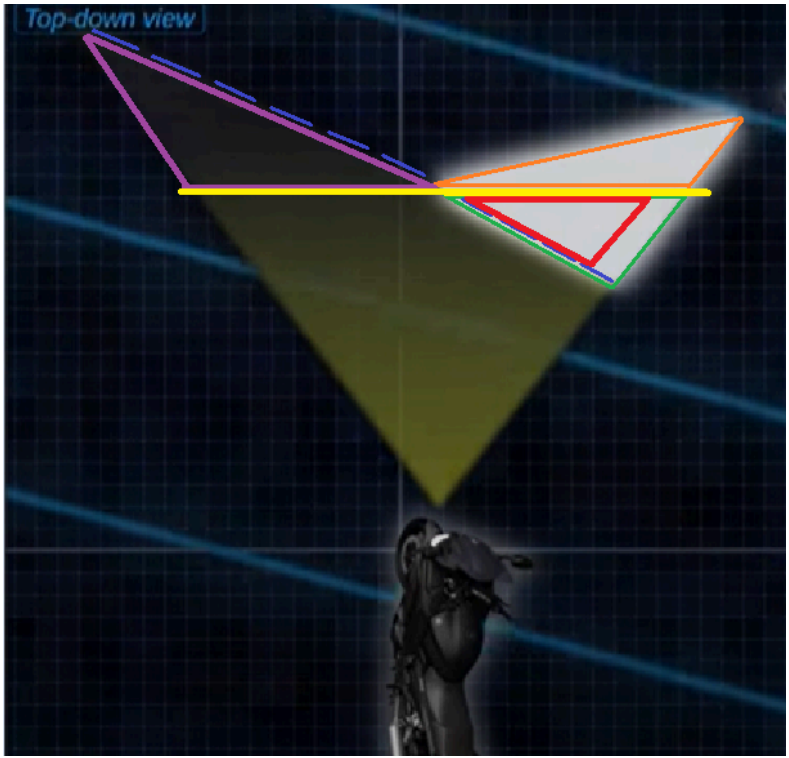
\includegraphics[width=0.75\linewidth]{Grafik/Cornering_Analysis_2.png}
    \caption{Lighting pattern changes with leaning at cornering}
    \label{cornering}
\end{figure}
\begin{itemize}
    \item \textbf{Yellow Line:} Horizontal line is the standard cut-off line when the motorcycle is level, which represents the transition between the high and low beam illumination zones
    \item \textbf{Blue Dashed Line:} Represents the low beam's horizontal alignment as the
    vehicle tilts, showing the change in the illumination pattern on the road. The
    area below this line is illuminated by the low beam, while the space above is
    illuminated by the high beam
    \item \textbf{Green Edged Triangle:} Represent the road section non-illuminated by low
    beam due to the vehicle's lean, requiring illumination for enhanced cornering
    visibility
    \item \textbf{Red Edged Triangle:} Represents the area illuminated by the pixel matrix high
    beam, limited compared to green triangle due to its matrix high beam’s narrower
    horizontal angle of illumination
    \item \textbf{Purple Edged Triangle:} Represents the area that must not be intensely
    illuminated to avoid causing glare, remaining non-adjustable due to the
    limitations of standard non-matrix low beams.
    \item \textbf{Orange Edged Triangle:} Represents the area that necessitates the application
    of an illumination gradient, guaranteeing a smooth fade-out from the light
    source to provide optimal visual comfort.
\end{itemize}

The principle of cornering compensation is designed to improve illumination on the side where the motorcycle is cornering. This means that as the motorcycle leans into a turn, the area of the apex, which typically suffers from poor lighting, receives enhanced illumination. This area is within the capabilities of the HD matrix's illumination range. The system's algorithm then activates specific pixels to project a triangular shaped light, effectively compensating for the lack of visibility in that area.  In the conclusion chapter effectiveness of the cornering compensation will be determined by error calculation method explain the \ref{method_error} ilumination coverage subchapter.

\subsection{Pitch Compensation Analysis}
Pitch compensation functionality of the motorcycle's headlight system is designed to address the change in the headlight beam's cut-off line that occurs when the motorcycle's nose dives during braking. The figure below offers a visual guide to how the lighting patterns change with braking at different pitch values. These changes are detailed in the bullet points that follow:
\begin{figure}[h!]
    \centering
    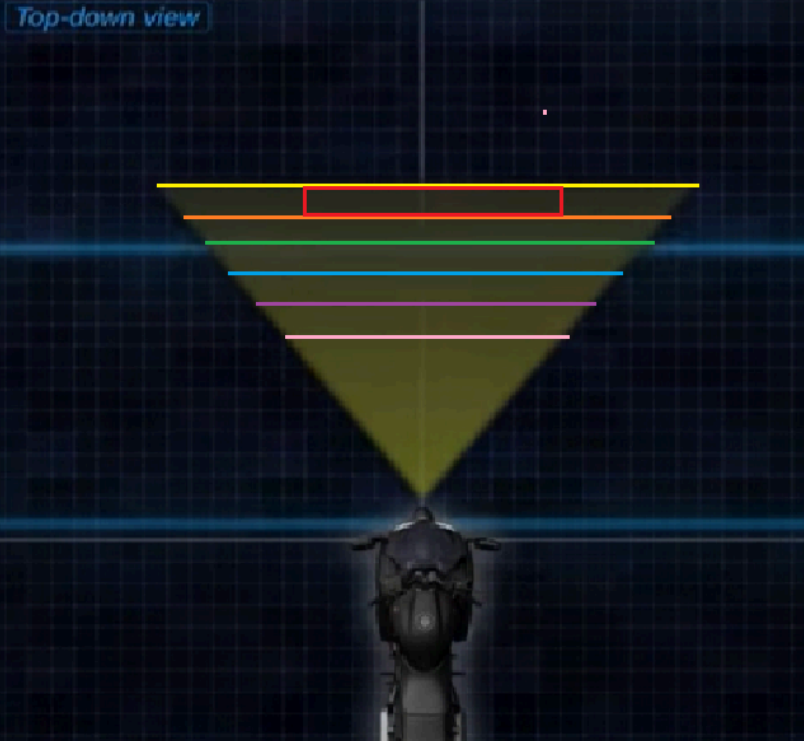
\includegraphics[width=0.75\linewidth]{Grafik/Pitch_Analysis_.png}
    \caption{Lighting pattern adjustments with braking at various pitch values}
    \label{pitch}
\end{figure}

\begin{itemize}
\item \textbf{0° Pitch - Baseline Illumination:} This is the standard cut-off line, represented
by the “yellow line” when the motorcycle is level, representing the transition
between the high and low beam illumination zones
\item \textbf{1° Pitch - Baseline Illumination:} Results in the cut-off line moving downward, a consequence of the
vehicle's nose dipping during braking, leading to a reduction in forward
illumination. The shifted cut-off line represented by the "orange line". The
red-edged rectangle illustrates the activation of a segment of the HD Matrix high
beam to counteract the minor downward displacement of the cut-off line caused
by the 1° pitch.
\item \textbf{Increased Pitch Angles:} As pitch angles increase, indicated by the green, blue, purple, and pink lines for 2°, 3°, 4°, and 5° pitches respectively, there's a corresponding downward shift in the cut-off line. This marks the transition from the upper boundary of the low beam to the lower edge of the high beam.
\end{itemize}

Consequently, pixel headlight system dynamically adjusts its illumination pattern with each pitch increment, where the upper edge of the illuminated area, marked by a red edge, moves upward to extend the light projection up to a yellow line, serving as the adjusted cut-off line. It calculates and compensates for the degree of pitch by activating the necessary pixels to maintain consistent visibility, effectively countering the dynamic cut-off line's displacement in real-time and ensuring enhanced road illumination 

In the conclusion chapter effectiveness of the cornering compensation will be determined by error calculation method explain the \ref{method_error} ilumination coverage subchapter


\subsection{Object Masking Analysis}
\textit{Currently waiting for a night ride with pixel headlight to get reference images}
%ADB ?


%% Re-consider the following



%\section{Methodology}
% Understanding requirements
% Feasibility Assesment
% System Design
% SW Development
% Verification And Validation

\begin{comment}
1. Understand the Requirements
		a. Safety concepts
			i. Performance levels PL (HARA)
			ii. Safety integrity levels
		b. Identify safety functions
			i. Overload protection
			ii. Emergency stop
			iii. Anti-collision system
			iv. Secure communication protocol
2. Risk Assesment
		a. Determine PL for each safety function
3. Design the System
		a. Select Appropriate components
			i. Harware, sensor, actuators
		b. System Architecture
4. Develop Safety-Related SW
		a. Adhere Guidelines
		b. Implement Safety Mesaures
			i. Safe state control, watchdog, error-handling 
Verification and Validation
\end{comment}


%%----------------------------------------------------------------------------
%% Theoretical part
	\chapter{System Description and Research}
\begin{comment}
Depending on the nature of the problem, this chapter should present the following briefly and in a way that the ideas for solutions, new concepts, process optimisation, results and conclusions can be understood and accepted by appropriately qualified readers:

consider here a chapter like sw dev with model based design 
reference: https://webthesis.biblio.polito.it/12441/1/tesi.pdf

>> detailed hw explain maybe also its hw arch
\begin{itemize}
	\item The theoretical basis used in your thesis
	\item Acknowledged methods of calculation and processes
	\item Methodological regulations and concepts (\eg VDI standard 2221 ``Methodological design'', TQM/TPM concept, ABC analysis, standards, \etc)
	\item Technological and physical foundation (material issues, manufacturing processes, physical laws, \etc)
	\item Economic methods and figures
	\item Legal basis
\end{itemize}
\end{comment}

\section{System Structure and Components}

The adaptive headlight software system is designed to dynamically adjust vehicle lighting, enhancing safety and visibility. At its core, the system leverages real-time telemetry inputs to assess vehicle dynamics, information about the driving environment  and driver inputs. These inputs are processed by the Light Control Unit (LCU), the decision-making hub equipped with advanced software.
\begin{figure}[h!]
    \centering
    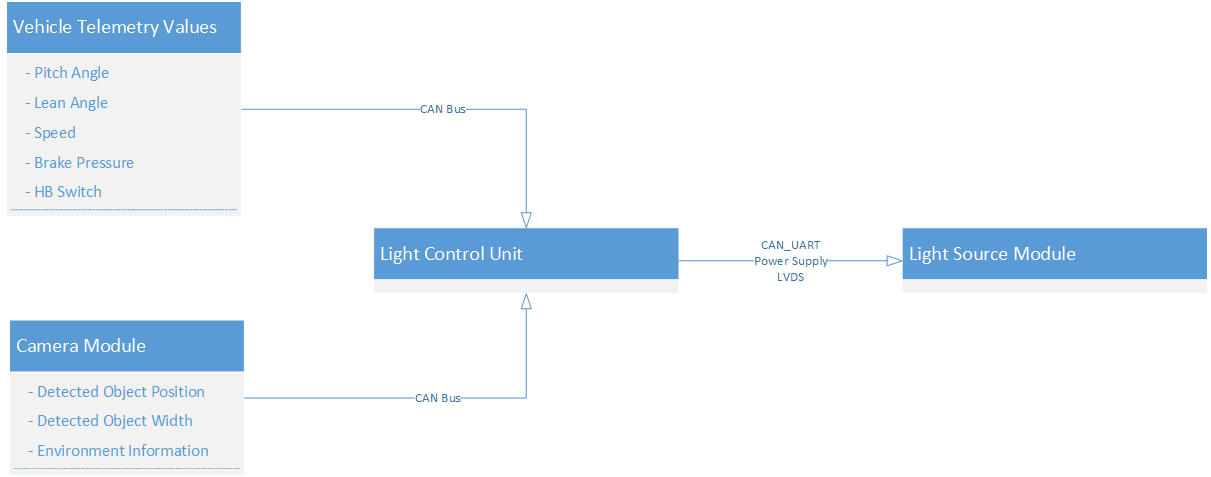
\includegraphics[width=0.75\linewidth]{Grafik/Overview_system_structure.png}
    \caption{The overview of the system structure}
    \label{fig:enter-label}
\end{figure}
The LCU orchestrates the operation of the Light Source Module (LSM), which utilizes HD matrix technology in the headlights. This technology allows for detailed adjustments in lighting patterns and intensity, tailoring illumination to suit varied driving environments and scenarios. Below is a simplified overview of the system structure, with further details provided in the following sections.
\subsection{Telemetry Values}
Telemetry inputs provide real-time data about the vehicle's movement and user inputs, enabling the system to adjust lighting conditions dynamically. Some of the main telemetry inputs used in the system include:

\begin{itemize}
    \item Lean Angle: Detects the side-to-side orientation of the vehicle.
    \item Pitch Angle: Detects the vehicle's front-to-back orientation.
    \item HB \& LB Signal: Tracks manual activation of high/low beams.
    \item Speed: Measures the vehicle's speed.
    \item Brake Pressure: Monitors brake activation.
    \item Ambient Light Sensor: Gauges external light levels.
\end{itemize}


These telemetry values are used in control logic to adjust each pixel, providing optimal illumination based on the current driving conditions.

\subsection{Camera Module}
To provide a glare-free high beam capability, vehicle detection is necessary to interpret traffic conditions. For this purpose, a camera module is mounted on the front of the motorcycle. This module includes the camera hardware, a software/firmware processing unit, and I/O interfaces that provide information via the CAN protocol. The key functionalities of the camera module for the adaptive headlight software are:

\begin{itemize}
    \item Object Detection: The system can detect up to 10 objects, categorizing them as either followed or approaching vehicles. To prevent glare, the pixels corresponding to these vehicles are completely shut off.
    \item Object Coordinates: Outputs the center coordinates and width of detected objects. The height is not considered as it does not impact road illumination.
    \item Environmental Information: Detects whether the vehicle is driven in specific conditions such as village areas, foggy conditions, or speed-limited zones. This information helps in providing Automated High Beam (AHB) functionality, particularly when the pixel HD matrix headlight is not available for mid and lower-end motorcycles.
\end{itemize}
In the following sections, the control software, logic, image creation, and system output, as well as detailing how these inputs are processed and utilized to optimize headlight performance will be discussed.


\section{Light Control Unit}
The Light Control Unit (LCU) serves as the core of the pixel headlight system, acting as both the system's brain and its central algorithmic processor. It processes real-time telemetry inputs, analyzes vehicle dynamics, and assesses environmental conditions to accurately modulate the headlight's output. The inputs to the LCU are CAN messages as previously mentioned. The output of the LCU is a grey-scale 2D array generated at each time step, with each element representing a pixel of the light source unit.

A software architecture and  UML diagram have been developed to optimally orchestrate the light source unit. The control software, flashed onto the LCU, incorporates the Ethernet Protocol (ETH) and User Datagram Protocol (UDP), ensuring reliable transmission of lighting commands to the light source unit.
The LCU's hardware includes dedicated PWM outputs for precise light intensity control, supporting Low Beam (LB) and High Beam (HB) headlights, each capable of handling up to 3 Amperes. This versatility allows management of Front Position Lamp (FPL) and Daytime Running Lights (DRL), with outputs rated at 200 milliamperes and 3 Amperes, respectively.

Additionally, the LCU features dual CAN interfaces for robust vehicle-wide communication and an LVDS interface for high-speed data or video signal transmission. These communication technologies are critical for exchanging control signals, enabling real-time lighting adjustments to meet the dynamic needs of the vehicle and its environment. This network of communication channels facilitates data transfer and integration between the LCU and the Light Source Module (LSM), enhancing interaction between the vehicle, driver, and environment while ensuring immediate lighting responses.

\section{Light Source Unit}
LSU in this project, also known as the HD Matrix LED Pixel
High Beam Headlight or simply 'pixel headlight,' is one of the main parts of the
vehicle's headlight system.

The input to the Light Source Unit (LSU) is a grey-scale image array integrated with the communication protocol (UDP+ETH), representing light illumination as processed by the software. The LCU uses telemetry data to direct the LSU to modify its lighting pattern, intensity, and direction, ensuring optimal adaptation to prevailing driving conditions. These continuous adjustments significantly enhance visibility and safety. Such continuous adjustments improve visibility and safety.

Key features of the LSU include:
\begin{itemize}
    \item Matrix Pixel LED Technology: Featuring a 64x256 matrix, the LSU houses 16,384 individually controllable LED pixels. This advanced technology allows for dynamic beam shaping, enhancing adaptability and safety in various driving environments. \cite{7_Internal_Doc_HELLA}
    \item SSL HD System: Utilizing Solid State Lighting (SSL) with High Definition (HD) capabilities, the LSU achieves detailed clarity and precision in its illumination pattern. This high-resolution technology ensures the light output is highly adaptable to different scenarios. \cite{7_Internal_Doc_HELLA}
    \item Beam Horizontal Angle: The SSL HD system provides various beam spreads, such as the "26°" model, offering a focused beam narrower than the average low-beam module. While this provides concentrated illumination, it also presents challenges in covering all areas typically illuminated by the low beam. \cite{7_Internal_Doc_HELLA}
\end{itemize}


Overall, the integration of the LSU with the LCU, supported by advanced lighting technology and real-time data processing, results in a headlight system that delivers optimal illumination tailored to real-time driving scenarios.







\section{Development for Embedded Applications}
% how to develop model-based systems for embedded applications
% 		○ Embedded environment,  Software engineer will often   directly to the microprocessor  without using a OS




\subsection{Characteristics of Embedded System}

\subsection{Real-Time Implementation}

\subsection{Code Generation and Deployment}








\newpage

\section{Vehicle Detection Algorithm}

\subsection{Overview}
\textit{". At present, the YOLO series is one of the most excellent algorithms in single-stage detection; it has the characteristics of a smaller parameter count, high detection accuracy, and high speed. Therefore, it is widely used in vehicle inspection"} \cite{Yolov5_Improvement}

\begin{figure}[h!]
    \centering
    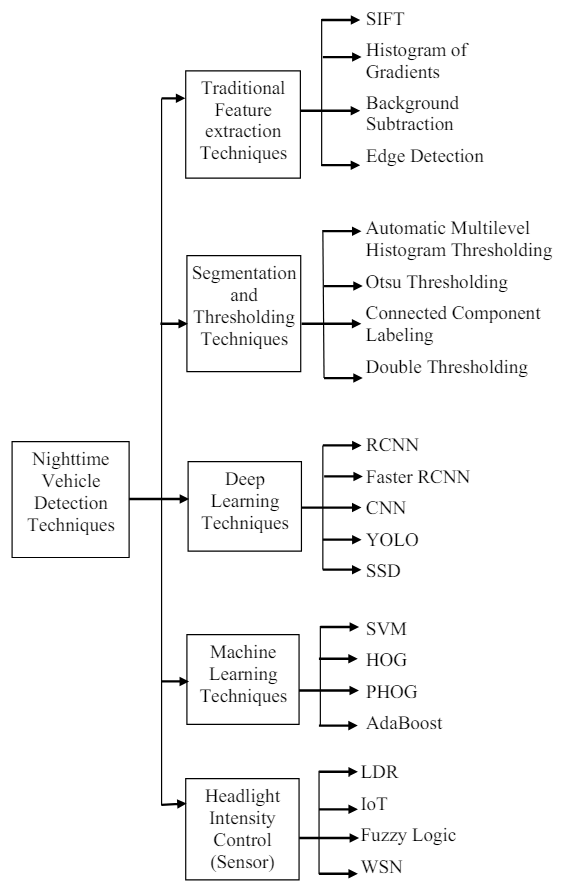
\includegraphics[width=0.75\linewidth]{Vehicle_detect_classification_nighttime.png}
    \caption{Classification of the techniques for nighttime vehicle identification and headlight intensity control. \cite{night_vehicle_detec}}
    \label{fig:enter-label}
\end{figure}


\subsection{Our Strategy - YOLOv5}

%https://www.mdpi.com/1424-8220/24/4/1182 \cite{Yolov5_Improvement}


\newpage
\section{Transformation Algorithm for Alignment}

\subsection{Rigid Body Transformation}

%%----------------------------------------------------------------------------
%% Method and practical part
	\chapter{Software Implementation}
\begin{comment}
This section deals in particular with your contributions to the thesis and may be subdivided into the following points, if necessary:

\begin{itemize}
	\item Analysis of current situation
	\item Results of patent reviews
	\item Description of state-of-the-art technology
	\begin{itemize}
		\item Review of literature with direct connection
		\item Information on existing solutions for aspects of the problem
		\item Discussion of the relevance with respect to your work
		\item Demonstration of your expertise in the area
		\item Factual presentation preferred
		\item Not just a listing of facts!
	\end{itemize}
	\item Presentation of target specifications for the actual state
	\item Calculations
	\item Tables and diagrams
	\item Concept development
	\item Principle sketches and/or construction drawings
	\item Prototype development
	\item Problem solution and test results (especially your contributions towards the problem solution; presentation of results as detailed as necessary):
	\begin{itemize}
		\item Analyses of initial situation and determination of approach to the problem
		\item Development of the concept and of the basic approach
		\item Detailed presentation of the development of solutions with all calculations, constructions, programme steps, tables and diagrams, \etc
	\end{itemize}
	\item Results, findings and innovation
	\item Evaluations, \etc
\end{itemize}	
The original ideas, innovations and technological developments must be explained and presented with appropriate detail.

\newpage
\subsection*{Discussion}
\begin{itemize}
	\item Discussion of approach, methods (pro and con)
	\item Results, findings and their discussion with respect to objectives
	\item Explanation of deviations
	\item Your opinion about the result
\end{itemize}

    
\end{comment}

\section{Software Architecture}

\section{Software Componets}
\subsection{Simulink Algorithm}
\subsection{Embedded C Interfacing}

\section{State Machine Logic}

\section{Model-Based Software Development}
\subsection{Welcome Home Function}
\subsection{Low Beam Enhancement Function}
\subsection{Object Masking Function}

\section{Hardware Integration and Deployment}

\section{Testing and Validation}
\subsection{Model Validation}
\subsection{Hardware-in-the-loop Testing}
\subsection{On-board Testing}
%%----------------------------------------------------------------------------
%% Conclusion
	\chapter{Conclusion}

\begin{comment}
This chapter should contain the following points:
\begin{itemize}
	\item Problem, aim (very briefly)
	\item Approach, problem solutions and concepts including their functional and/or technical and/or economic evaluation
	\item Short presentation of findings, central results, innovation of this work
	\item Conclusions and, if possible, prospect for future applications and development of solutions to meet the aim
\end{itemize}

    
\end{comment}

%%----------------------------------------------------------------------------
%% List of abbrevations[optional]
	\clearpage
	%\chapter{List of abbreviations [optional]}
\label{sec: Abbreviations}

\begin{table}[h]
	\centering
	\begin{tabular}{|p{3cm}|p{11.6cm}|}
		\hline
		\rowcolor{lightgray}\textbf{Abbreviation} & \textbf{Explanation} \\
		\hline
		& \\ 
		\hline
		& \\ 
		\hline
		& \\ 
		\hline
	\end{tabular}
\end{table}

\noindent The list of abbreviations \textbf{can} be used for a great number of abbreviations. List the abbreviations in the list in alphabetical order.

%%%+++++++++++++++++++++++++++++++++++++++++++++++++++++++++++++++++++++++++++
%% Latex bietet auch die Möglichkeit eines automatischen Abkürzungsverzeichnisses. Dieses entspricht aber nicht der Vorgabe und ist somit mit dem Betreuer abzusprechen.
%% In den folgenden Zeilen sind die nötigen Einstellungen angegeben und der Einfügebefehl angeführt.
%%%---------------------------------------------------------------------------
%% automatisches Abkürzungsverzeichnis
%%%---------------------------------------------------------------------------
%% In den TeXstudio-Einstellungen: 
%% ("Zeige erweiterte Einstellungen" muss aktiviert sein (In Einstellungsfenster: unten links))
 
%% 1. Schritt: Makeindex konfigurieren 
%%	- Reiter Befehle: 	Makeindex: makeindex.exe %.nlo -s nomencl.ist -o %.nls
 
%% 2. Schritt: Makeindex beim kompilieren ausführen 
%%	- Reiter Erzeugen:	Standardkompiler (rechts auf Schraubenschlüssel):
%%						makeindex zufügen 
%%%---------------------------------------------------------------------------

%% Abkürzungen hier einfügen:
%\abbrev{FH}{Fachhochschule}
%\abbrev{AT}{Automatisierungstechnik}

%\vspace{-41.5mm}
%\begin{minipage}{\textwidth}
%	\renewcommand{\nomname}{}
%	\printnomenclature
%\end{minipage}
%%%+++++++++++++++++++++++++++++++++++++++++++++++++++++++++++++++++++++++++++
%%----------------------------------------------------------------------------
%% Fachwortverzeichnis[optional]
	\clearpage
	%\chapter{Glossary [optional]}
\label{sec: Glossary}

\begin{table}[h]
	\centering
	\begin{tabular}{|p{3cm}|p{11.6cm}|}
		\hline
		\rowcolor{lightgray}\textbf{Term} & \textbf{Explanation} \\
		\hline
		 & \\ 
		\hline
		 & \\ 
		\hline
		 & \\ 
		\hline
	\end{tabular}
\end{table}

\noindent The glossary \textbf{can} be used for topics with a great number of specialist terms. This makes a definition within the text unnecessary and makes it easier for the reader to look them up (example: terms specific to the e-commerce area, \etc).
\vspace{6pt}\\
After completion, arrange the glossary in alphabetical order.

%%----------------------------------------------------------------------------
%% Abbildungsverzeichnis
	\clearpage
	\renewcommand{\listfigurename}{List of figures}
\listoffigures
\label{sec: ListOfFigures}
\chaptermark{List of figures}

%\noindent The list of figures \textbf{can} be used for a great number of figures.
%%----------------------------------------------------------------------------
%% Tabellenverzeichnis
	\clearpage
	%\renewcommand{\listtablename}{List of tables [optional]}
\listoftables
\label{sec: ListOfTables}
\chaptermark{List of tables}
\noindent The list of tables \textbf{can} be used for a great number of tables.
%%----------------------------------------------------------------------------
%% Formelverzeichnis
	\clearpage
	%\chapter{List of equations [optional]}
\label{sec: ListOfEquations}

\begin{table}[h]
	\centering
	\begin{tabular}{|M{0.8cm}|m{2.8cm}|m{10.8cm}|}
		\hline
		\rowcolor{lightgray}\textbf{No.} & \textbf{Name} & \textbf{Equation} \\
		\hline
		%\ref{eq: ExampleEquation-1} & Equivalence of mass and energy & $e=m\cdot c^2$ \\ 
		\hline
	\end{tabular}
\end{table}
\noindent The list of equations \textbf{can} be used for a great number of equations.
\vspace{6pt}\\
If necessary, copy the equations you used into this list of equations after completion of your thesis.

%%----------------------------------------------------------------------------
%% Bibliography
	\clearpage
	\chapter{References/Bibliography}
\label{sec: Bibliography}


Below you will find two sample references sections (bibliographies) covering the main types of publications (Internet source, standard, monograph, article in a book, technical rule, article in a specialist journal, AI tool). Information on other publication types can be found in ONR~12658 (for German) and in ISO~690 (for English), both of which are cited below. ONR~12658 and ISO~690 are available in the library of the Wels Campus and online, respectively.

\setlength{\parindent}{0mm}
\section{Bibliography for literature references within the text (AGR, AT, MB, PDK) or within a footnote (AMM, MEWI)}

\printbibliography[heading=none,env=bibliographyAlpha]
\nocite{*}

\vspace{1mm}
\fbox{\parbox{\textwidth}{In bibliographic software, predefined citation styles similar to this representation can be found via keywords such as “ISO 690”. 
Using such citation styles may necessitate manual modifications before you submit your thesis.}}


\section{Bibliography for literature references within the text (BI, BUT, IPM, LCW, LTE)}

Austrian Standards Institute (2013) \textit{ONR 12658:2013 Empfehlungen zum Zitieren von Informationsquellen und Anleitungen zur Gestaltung von Literatur- und anderen Quellennachweisen in wissenschaftlichen Arbeiten.}

\vspace{1mm}
Austrian Standards International (2023) \textit{ÖNORM A 2662:2023 Wissenschaftliche Abschlussarbeiten – Angaben für den bibliographischen Nachweis.}

\vspace{1mm}
Beuermann, C. (2013) \textit{Die Entdeckung des menschlichen Einflusses auf das Klima.} Available at: 
\texttt{https://www.bpb.de/gesellschaft/umwelt/klimawandel/38444/}
\texttt{entdeckung-des-menschlichen-einflusses} (accessed: 14 July 2021).

\vspace{1mm}
International Organization for Standardization (2021) \textit{ISO 690:2021 Information and documentation – Guidelines for bibliographic references and citations to information resources}.

\vspace{1mm}
Karmasin, M. und Ribing, R. (2019) \textit{Die Gestaltung wissenschaftlicher Arbeiten: Ein Leitfaden für Facharbeit/VWA, Seminararbeiten, Bachelor-, Master-, Magister- und Diplomarbeiten sowie Dissertationen.}
10\textsuperscript{th} edn. Wien: facultas.

\vspace{1mm}
Lehrndorfer, A. and Reuther, U. (2008) ‘Kontrollierte Sprache – standardisierte Sprache?{’}, in Muthig, J. (ed.) \textit{Standardisierungsmethoden für die Technische Dokumentation.} Lübeck: Schmidt-Römhild, pp. 97 121.

\vspace{1mm}
Meier, J. (2011) \textit{Globalisierung}. Wiesbaden: Pons.

\vspace{1mm}
Müller, E. and Meier, J. (2019) \textit{Globalisierung neu gedacht}. Wiesbaden: Pons.

\vspace{1mm}
Müller, E., Meier, J. and Huber, A. (2021) \textit{Globalisierung: Rahmenbedingungen, Prozesse, Institutionen}. Wiesbaden: Pons.

\vspace{1mm}
Müller, E., Meier, J., Huber, A. and Tausch, G. (2016) \textit{Globalisierung: Gegenwart und Zukunft}. Wiesbaden: Pons.

\vspace{1mm}
OpenAI (ed.) (2023) ChatGPT, version xy [language model]. \textit{Response to the author’s prompt “xyz”}, generated 1 December 2023. Available at: \newline 
\texttt{https://chat.openai.com/} (accessed: 1 December 2023).

\vspace{1mm}
Schulz, M. (2014) ‘Doku-Norm in der Praxis’, \textit{technische kommunikation}, 36(6), pp. 46-49.

\vspace{1mm}
\fbox{\parbox{\textwidth}{In bibliographic software, predefined citation styles similar to this representation can be found via keywords such as “cite them right”. 
Using such citation styles may necessitate manual modifications before you submit your thesis.}}
--

\section{Bibliography for numeric references in square brackets (AB, AET, AGR, AMM, AT, BUT, EE, LTE, MB, MEWI, RSE, SES, VTP, WFT)}
\printbibliography[heading=none]

\vspace{1mm}
\fbox{\parbox{\textwidth}{In bibliographic software, predefined citation styles similar to this representation can be found via keywords such as “ISO 690”. 
Using such citation styles may necessitate manual modifications before you submit your thesis.}}

\newpage
\section*{Appearance}
%The appearance of the bibliography varies depending on the reference style that you must apply in your thesis [see section \ref{sec: TypeOfCitation} on page \pageref{sec: TypeOfCitation}].

\section*{Division}
The list of references can be sub-divided into the following sub-sections, if necessary:
\begin{itemize}
	\item	Primary literature 
	\item	Secondary literature
	\item	Tertiary literature
\end{itemize}

\section*{Literature search}
On the Internet pages of the library of the Wels Campus, you can find a very detailed list with numerous links to:
\begin{itemize}
	\item	electronic journals
	\item	databases
	\item	numerous libraries
	\item	catalogues of the book trade
	\item	patent agencies

\end{itemize}
The library staff are happy to help you with your literature search.


%%----------------------------------------------------------------------------
%% Appendix[optional]
	%\chapter{Appendix [optional]}
The appendix contains supplements such as regulations, instructions, detailed data, detailed design drawings, \etc, if they are necessary to improve understanding of the context.
%%----------------------------------------------------------------------------
%% Checkbox of the printed size
	%\chapter*{Release and printing size information}
\thispagestyle{plain}
This page is used to check the version of the style and frontpage packages used and to check the scaling factor of the printout.\\
\rule{15cm}{0.3mm}
\begin{center}
	{\Large --- Check the release! ---}\\
	{\small \url{https://www.fh-ooe.at/campus-wels/}}\\
\end{center}
\begin{tabbing}
	\hspace{4cm}\=\hspace{4.5cm}\=\kill
	\>{\large --- Main file:}\>{\CurrentVersionMain ---}\\ 
	\>{\large --- Style package:}\>{\CurrentVersionStyle ---}\\ 
	\>{\large --- Frontpage package:}\>{\CurrentVersionFrontpages ---} 
\end{tabbing} 
\rule{15cm}{0.3mm}
\begin{center}
	{\Large --- Check the page margins! ---}
\end{center}
\begin{flushleft}
	| left margin
\end{flushleft}
\vspace{-2.875\baselineskip}
\begin{flushright}
	right margin |
\end{flushright}
\vspace{-\baselinestretch\baselineskip}
\rule{15cm}{0.3mm}
\begin{center}
	{\Large --- Check the scaling factor of the printout! ---}\\
	\bigskip
	\Messbox{100}{50}
\end{center}
\rule{15cm}{0.3mm}
\begin{center}
	{\Large --- Remove this page after printing! ---}\\
	\quad\newline
	{\Large --- In case of electronic submission, this page has to be removed from the {\LaTeX} document! ---}
\end{center}
\rule{15cm}{0.3mm}
%%============================================================================	
\end{document}
%%++++++++++++++++++++++++++++++++++++++++++++++++++++++++++++++++++++++++++++